%%%%%% General %%%%%%%%%%%%%%%%%%%%%%%%%%%%%%%%%%%%%%%%%%%%%%%%%%%%%%%%%%%%%%{{{
\chapter{Background}\label{sec:general}

This chapter describes the terms, techniques, tools and programs used during the
work for this thesis. It provides a general overview to make it easier to
understand the details of the work in the following chapters. We start by
showing how modern computers execute programs and code, by looking at file
formats needed to load programs and how common computing architectures structure
their machine code. We then look at how programs and code is tested and what new
technologies evolved in that matter. As we deal with Unix based systems, we take
a look at the permission system used by those.
Additionally, we face topics in secure communication. Therefore we also describe
the basic principles of network connections, web servers and their security. The
thesis provides automation for searching for bits to flip with rowhammer,
because of this we take a look at this kind of attack and how it works and also
look at microarchitectural attacks in general.

\section{Executing Programs}

Processing units (PU) execute machine code. Any device running programs contains
at least one. Usually, the central processing unit (CPU) runs programs and
triggers other PUs to run other tasks if needed. Often referred to as the main
processor, the CPU carries out the instruction given to it by the machine code
representing a program. A PU can only step over single instructions and execute
them one by one. This is done by moving the instruction pointer to different
memory locations. Simple processors may only execute one single program. On
ordinary desktop computers, the operating system is the main program which can
load other programs as processes and manage them. CPUs can only execute machine
code, but programs usually are written in programming languages which are then
translated to machine language by either a compiler or an interpreter. We refer
to files created by a compiler as executables or binaries. These files can
directly be loaded into memory by the OS. Operating Systems use defined
structures for executables to make this loading possible, for example,
Unix/Linux systems use ELF and Windows uses PE.

\subsection{CPU Instructions}

Machine code, in general, is a list of instructions, encoded in some binary
format. Usually, an instruction consists of an operation code (opcode), telling
the processor what to do, and parameters for the opcode, which the processor
uses for the operation. Instructions can operate on registers or locations in
memory directly. Available instructions and their design are depending on the
architecture used. The most common instruction set architectures (ISA) are Intel
$x86$, mostly referred to as \texttt{x86\_64} or \texttt{AMD64}, and ARM ISA
which is used by most mobile processors.

\begin{table}[]
\begin{tabular}{ccccccc}
\cline{2-7}
\multicolumn{1}{c|}{} & \multicolumn{1}{c|}{Prefix} &
\multicolumn{1}{c|}{Opcode} & \multicolumn{1}{c|}{ModR/M} &
\multicolumn{1}{c|}{SIB} & \multicolumn{1}{c|}{Displacement} &
\multicolumn{1}{c|}{Immediate} \\ \cline{2-7}
bytes         & 1 per prefix                & 1, 2 or 3
 & 0 or 1                      & 0 or 1                   & 0, 1, 2 or 4
             & 0, 1, 2 or 4
\end{tabular}
\caption{Instruction Format for Intel 64 and IA-32 architectures. It shows how
many different instruction lengths are possible in modern architectures and
also which parts they may contain.}
\label{tab:instrfor}
\end{table}

Table~\ref{tab:instrfor} shows the instruction format for Intel 64 and IA-32
Architectures. The format splits an instruction into the following sections:

\begin{itemize}
  \item Prefix - Used to give the CPU further instructions on how to handle the
opcode. There are prefixes for memory locks in a multi-core environment or
repeat instructions to apply an operation on each byte in a string or I/O data.
There are also prefixes overriding the operand sizes or introducing SSE
instruction calls, or even others give branching hints to the CPU.
  \item Opcode - Tells the CPU what to do and how to handle the following
parameters.
  \item ModR/M - This byte is used behind the opcode to tell the CPU what
addressing mode to use for memory accesses.
  \item SIB - For some ModR/M addressing-modes, this byte also needs to be
parsed and evaluated.
  \item Displacement - Some addressing-modes referred in the ModR/M or SIB byte
might include a displacement following them.
  \item Immediate - Immediate data might follow if referred in previous
parameters.
\end{itemize}

We refer to the Intel Manual~\cite{intelsys} section 2.1 for further details on
the instruction format used in \texttt{x86\_64}.

\subsection{Executable and Linkable Format (ELF)}

ELF is an object file format. It is used to describe a program in a way to load
a program into memory to make it execution ready for the processor without
applying changes to the binary itself. A linker creates ELF files after an
assembler turned the program's source code into machine code. Most modern
Unix-like operating systems follow the ELF specification released by the Tool
Interface Standard Committee~\cite{elfspec}. Therefore, we need to understand
the layout of such executable files before introducing bitflips to them.

\subsubsection{Structure of an ELF file}

\tikzstyle{block} = [rectangle, minimum width=2cm, minimum height=0.8cm,
text centered, draw=black]
\tikzstyle{dot} = [circle, fill, inner sep=1.5pt]
\tikzstyle{function} = [rectangle, rounded corners, minimum width=2cm,
minimum height=0.8cm, text centered, draw=black, fill=blue!30]
\tikzstyle{arrow} = [thick,->,>=stealth]
\tikzset{XOR/.style={draw,circle,append after command={
        [shorten >=\pgflinewidth, shorten <=\pgflinewidth,]
        (\tikzlastnode.north) edge (\tikzlastnode.south)
        (\tikzlastnode.east) edge (\tikzlastnode.west)
        }
    }
}
\tikzstyle{level3block} = [rectangle, minimum width=9.5cm, minimum
height=0.8cm, text centered, draw=black]
\tikzstyle{mcblock} = [rectangle, minimum width=4cm, minimum
height=0.8cm, text centered, draw=black]
\tikzstyle{doublearrow} = [thick,<->,>=stealth]
\tikzstyle{segblock} = [rectangle, minimum width=1cm, minimum height=0.8cm,
text centered, draw=black]
\tikzstyle{memarray} = [rectangle, minimum width=3cm, minimum height=3cm,
                        text centered, draw=black]
\tikzstyle{memfunc} = [rectangle, minimum width=3cm, minimum height=1cm,
                       text centered, draw=black]
\tikzstyle{memcon} = [rectangle, minimum width=2cm, minimum height=2cm,
                        text centered, draw=black]
\tikzstyle{line} = [thick,-,>=stealth]

\begin{figure}
  \centering
  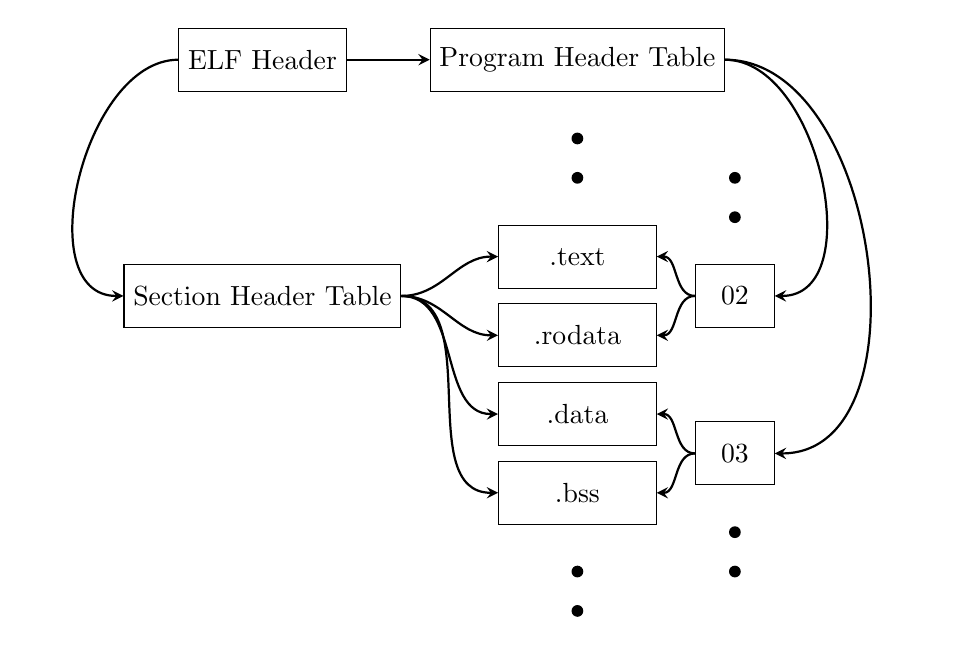
\begin{tikzpicture}
  \node (eh) [block] {ELF Header};
  \node (ph) [block, right of=eh, xshift=3cm] {Program Header Table};
  \node (sh) [block, below of=eh, yshift=-2cm] {Section Header Table};
  \node (dot0) [dot, below of=ph] {};
  \node (dot1) [dot, below of=dot0, yshift=0.5cm] {};
  \node (text) [block, below of=dot1] {.text};
  \node (rodata) [block, below of=text] {.rodata};
  \node (data) [block, below of=rodata] {.data};
  \node (bss) [block, below of=data] {.bss};
  \node (dot2) [dot, below of=bss] {};
  \node (dot3) [dot, below of=dot2, yshift=0.5cm] {};
  \node (seg02) [segblock, right of=text, xshift=1cm, yshift=-0.5cm] {02};
  \node (dot4) [dot, above of=seg02] {};
  \node (dot5) [dot, above of=dot4, yshift=-0.5cm] {};
  \node (seg03) [segblock, right of=data, xshift=1cm, yshift=-0.5cm] {03};
  \node (dot6) [dot, below of=seg03] {};
  \node (dot7) [dot, below of=dot6, yshift=0.5cm] {};
  % connections
  \path [thick,->,>=stealth] (eh) edge[out=0, in=180] (ph);
  \path [thick,->,>=stealth] (eh) edge[out=180, in=180] (sh);
  \path [thick,->,>=stealth] (sh) edge[out=0, in=180] (text);
  \path [thick,->,>=stealth] (sh) edge[out=0, in=180] (rodata);
  \path [thick,->,>=stealth] (sh) edge[out=0, in=180] (data);
  \path [thick,->,>=stealth] (sh) edge[out=0, in=180] (bss);
  \path [thick,->,>=stealth] (ph) edge[out=0, in=0] (seg02);
  \path [thick,->,>=stealth] (ph) edge[out=0, in=0] (seg03);
  \path [thick,->,>=stealth] (seg02) edge[out=180, in=0] (text);
  \path [thick,->,>=stealth] (seg02) edge[out=180, in=0] (rodata);
  \path [thick,->,>=stealth] (seg03) edge[out=180, in=0] (data);
  \path [thick,->,>=stealth] (seg03) edge[out=180, in=0] (bss);
  \end{tikzpicture}
  \caption{Structure of an ELF file showing the four main sections inside an
executable. The Figure shows the connection of between sections and segments via
the program header table and the section header table. Segments usually are just
numbers and can refer to multiple sections inside the section header table.}
\label{fig:elfstruct}
\end{figure}

There are two views of an ELF file, the linking view and the execution view.
Those are also called section and segment view respectively. They share the same
ELF header but serve different purposes for the operating system. Figure
~\ref{fig:elfstruct} show the connection between sections and segments via the
two different headers. Sections and segments can be seen as follows:

\paragraph{Sections} describe the binary for the linking view. A section
contains instructions, data, symbol table and relocation information. Sections
reserved for the system start with a dot, there might be additional sections
defined by the user. Sections are created and managed by the linker. Sections
that are directly loaded into the program's memory image are initialized data
(\texttt{.data, .data1}), read-only data (\texttt{.rodata, .rodata1}) and
executable instructions (\texttt{.text}).

\paragraph{Segments} describe the virtual memory layout of a loaded binary.
Figure~\ref{fig:elfstruct} shows how segments are applied in an ELF file.
Usually, the linker splits segments into different behaviours the loader needs
to apply. For example, all read-only data sections are in the same segment. When
loading the image into memory references inside the ELF file need to be resolved
and loaded into the memory too. After successfully loading the image and its
dependencies the program can be executed.

\subsubsection{Loading ELF files into Memory}

As we focus on GNU/Linux operating systems, we will look at how UNIX System V
Release 4 based operating systems handle ELF files in order to create running
programs. Operating systems use no physical addresses for execution, and the OS
is free to change the position of sections in the virtual address space.
Therefore, in an ELF, a section only contains a base address and offsets to that
address. During the loading step, the operating system is free to change the
base address in the programs virtual address space. The loader then places
additional memory according to these offsets.

\paragraph{Dynamic Linking} is needed because it is widespread to have multiple
functions used by different programs. Shared libraries can be used to provide
such general functions. When deploying programs, developers usually make sure
all needed shared libraries exist on the target platform or ship their software
with those included. When depending on libraries by the system, the loader will
move the shared libraries into memory at the desired entry point. The loader
fetches the information about the needed library from the ELF file and then
checks the library paths provided by the operating system if the library is
available to be loaded.

\section{Analysis and Testing of Executables}

Testing is a significant part of software development. There are a lot of
different approaches and styles for testing. One approach to test a program is
to apply input to it and check if the code operates as expected by validating
the output. With increasing amount of code and an increasing number of bugs
found, the style of testing changed over the years. On the one hand, developers
nowadays provide unit tests inside their code to test single functions and make
sure they work as desired. On the other hand, sometimes the source code is not
available to a tester, or it is way too much work to read the whole source code
to such tests. Therefore, developers came up with tools which can be used to
test binaries on their own without knowing the source code.

\subsection{Fuzzing}

Fuzzing is an approach for testing programs with just a little knowledge about
the program to test. Such an approach is called black box testing. Fuzzing is a
technique to detect erroneous responses of a program by providing different,
automatically created, mostly random, inputs. Tools applying this technique are
called fuzzers. Fuzzers try to reach corner cases in programs without knowing
which exist and detect undefined behaviour or crashes. Generally, fuzzers give
an overall view on the robustness of a program, they are cheap to apply and even
can find bugs usual white box tests would miss.

If a fuzzer only applies random inputs, testing would take a very long time, as
a lot of unneeded tests would run. Because of this, the technology improved over
the time and different fuzzers evolved. For simple programs just testing common
input mistakes, like negative numbers, newlines, end of file characters, format
strings or just very long strings might be enough. Advanced software needs
better ways of fuzzing, for example, network protocols, file systems or image
formats have a very complex structure which makes it hard to find possible
crashes by random data input. Fuzzers for such kind of software generate inputs
from given examples and apply small changes to them. Like,
Xmlfuzzer~\cite{xmlfuzzer} is a tool crafted specially to test XML schemes in
programs. Besides special format fuzzers, more advanced ones exist which
directly interact with the target, allowing to track execution paths per input
and therefore even create more test cases automatically. The most popular fuzzer
is "american fuzzy lop" (afl)~\cite{aflweb}. It contains described algorithms to
get the best possible code coverage. Another more advanced fuzzer is Steelix by
Yuekang~\etal~\cite{steelix}, which provides program-state based binary fuzzing.
Steelix uses static-analysis and binary instrumentation to provide more
information about the fuzzing process and therefore gains better test cases and
execution paths for the fuzzed program. Shoshitaishvili~\etal showed how fuzzing
could find authentication bypasses in binary firmware with their tool
Firmalice~\cite{firmalice}. In their work Wang~\etal~\cite{inmemfuzzing} showed
how in-memory fuzzing is used to detect similarities in binary code. This is
done by fuzzing every function available and compare traces of program
behaviours with machine learning models. They show that they can find
similarities in binaries even when different compilers, optimisations or
obfuscation is applied.

\subsection{Symbolic Execution}

Fuzzing provides a pseudorandom input to a program to test it. Therefore it
might not catch all possible execution paths of a program. Scientists developed
techniques to test all possible paths by simplifying the program,  one of this
techniques is symbolic execution. It makes use of the possible simplification of
inputs where they use a logic symbol with less possible states instead. For
example, a number can be represented by the possible states: maximal value,
minimum value, positive, negative, zero. The possible symbolic-state inputs then
run through the program in combination with a constraint solver to report
possible violations of the program's specification. The solver can also be used
to find possible paths to reach a pre-defined goal inside the binary.

One of the most famous symbolic analysis frameworks is angr~\cite{angrpaper}.
Besides the symbolic execution of binaries, it also allows various other
analysis methods such as control-flow graph recovery, automatic exploit
generation or automatic binary hardening.

Stephens~\etal~\cite{driller} showed with Driller how symbolic execution could
be beneficial to fuzzing approaches. This allows keeping the number of execution
paths to test lower but also try to cover as much code as possible. Driller uses
concolic execution for the path exploring. Concolic execution is the combination
of symbolic and concrete execution of a program.

\subsection{Instrumentation}

Instrumentation comes down to adding new code to already existing one in an
automated manner. Developers use instrumentation as a tool for debugging or
performance measures by adding calls to timing functions or information logging
to the code. Information from instrumentation could be something like what
functions are called and how often, what execution branches are taken, how long
does a subroutine take, what memory is accessed and many more. It usually also
allows the developer to change the runtime environment of a program, like change
return values or skip instruction calls.

Two different styles of instrumentation exist, one is source instrumentation,
and one is binary instrumentation, where so-called instrumenter-calls are either
added pre-compilation to the source of the program or later added to the binary
context of the program. The first style might bring the advantage that it is
easier to apply and the structure of the program is better known to the
instrumenter, so calls for performance checks over functions are done by adding
timer calls at the entry and exit points. However, binary instrumentation also
has its perks. For example, users do not need the source of the program, which
might not be available in proprietary programs. Also, recompilation of the
program is not needed if the code for the instrumentation changes. Given enough
debug information in the binary the instrumentation information might not differ
much from the source based one. With binary instrumentation it is also possible
to change and read register values before and after CPU instructions are called,
which might not be possible at source code level, as used registers and memory
areas are unknown to the instrumenter at this point.

\subsubsection{Intel Pin}

Pin~\cite{pintool} is a proprietary, dynamic, binary instrumentation framework
developed and released by Intel, who supply it for free. The framework provides
a large number of API calls which abstracts most of the work done by Pin and
gives easy access to binary analysis. As Pin is a binary instrumentation
framework, the source of the to be analysed program is not needed, and the
program does it need to be recompiled if the instrumentation tool changes. The
framework allows to log and modify the runtime of a program, whereas it is no
problem to log register values or change those before or after desired
instruction calls or even inject code to be run before given calls. Programs
instrumenting a binary are called pintools, the framework provides their API
calls for C++, but also bindings for Python can be found in
\texttt{python-pin}~\cite{pythonpin}.

\section{Permission Model in Unix-based Systems}

The POSIX standard~\cite{posix} defines many properties for operating systems,
also permissions for users and their groups. For practical reasons, a user can
be part of multiple groups. A unique integer ID per user and group provides
identification to the system. The POSIX-defined permission structure applies to
files, which can have properties like readable, writable, executable. On
creation, the user can set these properties separately for the owner, the group
of the owner and others. POSIX also allows users with special privileges to
suppress such permission checks. These users are called super-users.

Besides permission for files most Unix based systems also provide permission
checks for processes and their owner. For example, only processes owned by a
super-user might be allowed special syscalls. In most systems, only one
super-user exists, namely \texttt{root}. Usually, users do not want to login
another time if they need super-permissions for a task. Therefore, POSIX
compliant operating systems ship tools such as \texttt{su} or the more advanced
\texttt{sudo}. \texttt{su} stands for switch user and allows a user to change
the current context to another user or execute a command with the other user's
permissions, providing the correct password of the other user. \texttt{sudo}
includes the same functionality as \texttt{su}. Additionally, it has a better
management system in the background and given the correct permissions the user
does not need to know the other user's password to execute commands as the
target user.

\subsection{\texttt{setuid} Binary Property}

\texttt{setuid} stands for "set user identity"~\cite{ogroupsetuid}. It allows an
executable to change its user ID on execution. An additional bit in the file
permissions represents the \texttt{setuid} property, namely \texttt{S\_ISUID}.
This property allows a user to run a program with the permissions of the file's
owner. Tools like \texttt{su} and \texttt{sudo} need this as they require the
permission to change the current context. It is also practical to allow normal
users the usage of tools like \texttt{ping} or \texttt{ip}, without allowing
them to use \texttt{sudo}. We refer to the GNU libc documentation for more
details~\cite{libcpermission}.

Whereas the \texttt{setuid} property might seem practical, it also brings
security risks. A bug allowing code execution in such a program allows an
attacker to execute that code with the permission of another user. Therefore,
the number of \texttt{setuid} binaries should be low and programs having that
property should be well audited.

\section{Connecting Computers}

People are exchanging data between devices for several decades now. The Internet
started when scientists found a way to have universities share research results
between computers over the back then used Advanced Research Projects Agency
Network (ARPANET).  The ARPANET already used the TCP/IP protocol and showed
requirements for future interconnection networks. With easier access to
computers, more universities, companies and private households wanted to be
connected and exchange data. Many protocols were introduced with the creation of
the Internet, where Hypertext protocols are shared in the World Wide Web,
electronic mail is used to transmit messages, and file sharing became common.
With this growing amount of users, security in the network and the connected
devices became more relevant every day. Therefore, protocols to ensure security
for the participants became standard and regularly improved.

\subsection{Webserver}

Web servers provide users with content on the Internet, mostly referred to as
the World Wide Web (WWW). There are many different software implementations for
such servers available, most of them being open source and free, such as
Apache\cite{apacheweb} and \texttt{nginx}\cite{nginxweb}. Web servers use the
Hypertext Transfer Protocol (HTTP) to handle requests and deliver the content to
the client. Web servers usually deliver websites encoded in Hypertext Markup
Language (HTML) but can also deliver all kind of files such as JavaScript (JS)
and Content Style Sheet (CSS).

A client requests content from the server by sending a Uniform Resource Locator
(URL). The server then looks up the given path in the URL and answers the
request by sending the desired file or an error if one occurs during the
handling of the request. As not all requests should publicly visible web servers
adapted TLS for security and privacy reasons to provide content over HTTPS. The
client, most of the time a web browser, can thereby verify the server's identity
and apply encryption to the connection if needed.

\subsubsection{HTTP - Basic Access Authentication (BA)}

To allow only authorised users to access specified paths on a web server HTTP
added access-control to the protocol described in RFC 7617~\cite{rfc7617}. This
technique makes use of a header field in HTTP, namely \texttt{WWW-Authenticate}.
RFC 3986~\cite{rfc3986} deprecates the functionality to transmit credentials
inside the URL. BA is a straightforward access-control technique and does not
protect the transmitted credentials. Therefore, it is used together with HTTPS
at most times. The client has to transmit the credentials with every request,
and there is no logout function as in other techniques using cookies or session
identifiers.

\paragraph{Access control in Apache and \texttt{nginx}} is done by providing
Basic Access Authentication in the default configuration. Apache makes use of
\texttt{ht} files, which are an extension to the usual server configuration for
users with limited rights, see their documentation~\cite{apacheauthdoc} for
further details. Apache introduced \texttt{htpasswd}-files to make use of BA,
which stores the user credentials. \texttt{nginx} later adapted these files for
their web server implementation. The \texttt{htpasswd}-files keep the data
either in plaintext or hashed. To create these files Apache provides the tool
\texttt{htpasswd}~\cite{htpasswddoc}. This tool uses MD5 hashing per default (as
of version 2.2.18), but it is possible to change the hashing algorithm to
something more secure. On a request including BA, the web server will look up
the \texttt{htpasswd}-file to verify given credentials and then return the
requested content or an error according to RFC 7231\cite{rfc7231}.

\subsection{Transport Layer Security}

Transport Layer Security (TLS) describes a collection of cryptographic
protocols. It is a standard proposed by the Internet Engineering Task Force
(IETF), RFC 5246\cite{rfc5246} describes the standard in detail. The IETF
regularly updates the TLS standard by adding new protocols and removing old,
seen as insecure, ones.

TLS provides a secure connection between various devices, usually clients and a
server. The connection holds the following properties:
\begin{itemize}
  \item Authenticated identities are provided by public-key cryptography. This
is needed for clients to make sure they communicate with the correct server. TLS
certificates provide the ability to prove the identity of a server. Protocols
use the certificates as they contain the public key of the server.
  \item Private connections between the parties are provided by symmetric
cryptography. The participants in a connection have to agree on how they
exchange the key for the symmetric encryption.
  \item Reliability is provided by the so-called message authentication code
(MAC), which prevents undetected alteration or losses during TLS communication.
\end{itemize}

As TLS is just a collection of protocols, the parties have to agree on which one
they use for each part of the connection, which happens during the TLS
Handshake. A common name for a TLS connection protocol would be
\texttt{ECDHE-RSA-AES256-GCM-HMAC-SHA1}, which contains all three protocols used
for the connection. Whereas \texttt{ECDHE-RSA} provides the key exchange,
\texttt{AES256-GCM} is the  symmetric cypher and \texttt{HMAC-SHA1} checks data
integrity.

TLS is commonly used in web servers to guarantee user's safety, but also
applications like Virtual Private Networks (VPNs) and Secure Shell (SSH) make
use of protocols and cyphers described in the TLS standard. The most commonly
used TLS implementation is OpenSSL~\cite{opensslweb}.

\subsection{Cryptographic Nonces}

In the early days of encrypted communication, replay-attacks were a common
problem, as Syverson showed in his taxonomy of replay attacks in
1994~\cite{replaytax}. Newer protocols introduced nonces to resolve this issue.
Cryptographic nonces are one-time, often pseudorandom, numbers used for each
packet sent. They are combined with the key so that the encryption differs for
each packet. This technique makes replay-attacks harder.

In most cases, nonce reuse is a problem for the protocol and results in breakage
of the encryption of future or past packages. Hence, most protocol standards
define a nonce as a pseudorandom, non-repeating or unpredicted
value~\cite{noncegeneral}. It is also possible to use the nonce as a counter
which has a random start value and increases for each packet sent. However, also
current protocols and technologies still face problems with nonces, like
Vanhoef~\etal showed in their work in 2017, that it is possible to force nonce
reuse in WPA2\cite{wpanoncereuse}.

\subsection{AES-GCM}

Galois Counter Mode (GCM) in combination with Advanced Encryption Standard (AES)
provides encryption and simultaneously performs message
authentication~\cite{gcm, gcmnist}. Figure~\ref{fig:aesgcm} shows the schematic
of AES-GCM. Where we use close to the same notation as Böck~\etal in their
paper~\cite{gcmnonceattack}:

\begin{itemize}
  \item[$CNT_i$] The $i$-th counter block, computed using the concatenation of
the $IV$ and the counter value $cnt$, $cnt = (i+1) \mod{2^{32}}$, to achieve 128
bits. $CNT_0 = IV \parallel 0 ^{31} \parallel 1$. With $IV$ being the
initialisation vector with a size of 96 bits.
  \item[$E_k$] AES encryption with symmetric key $k$.
  \item[$a \oplus b$] XOR operation between $a$ and $b$.
  \item[$P_i$] The $i$-th plaintext block.
  \item[$C_i$] The $i$-th ciphertext block.
  \item[$mult_H$] Multiplication $H \cdot X$ in Galois Field GF($2^{128}$),
with the irreducible polynomial $g = g(x) = x^{128} + x^{7} + x^{2} + x + 1$.
  \item[$A$] Authenticated data.
  \item[$len(X)$] Bit-length of $X$.
  \item[$a \parallel b$] Concatenation of $a$ and $b$.
  \item[$TAG$] Authentication tag.
\end{itemize}

\begin{figure}
  \centering
  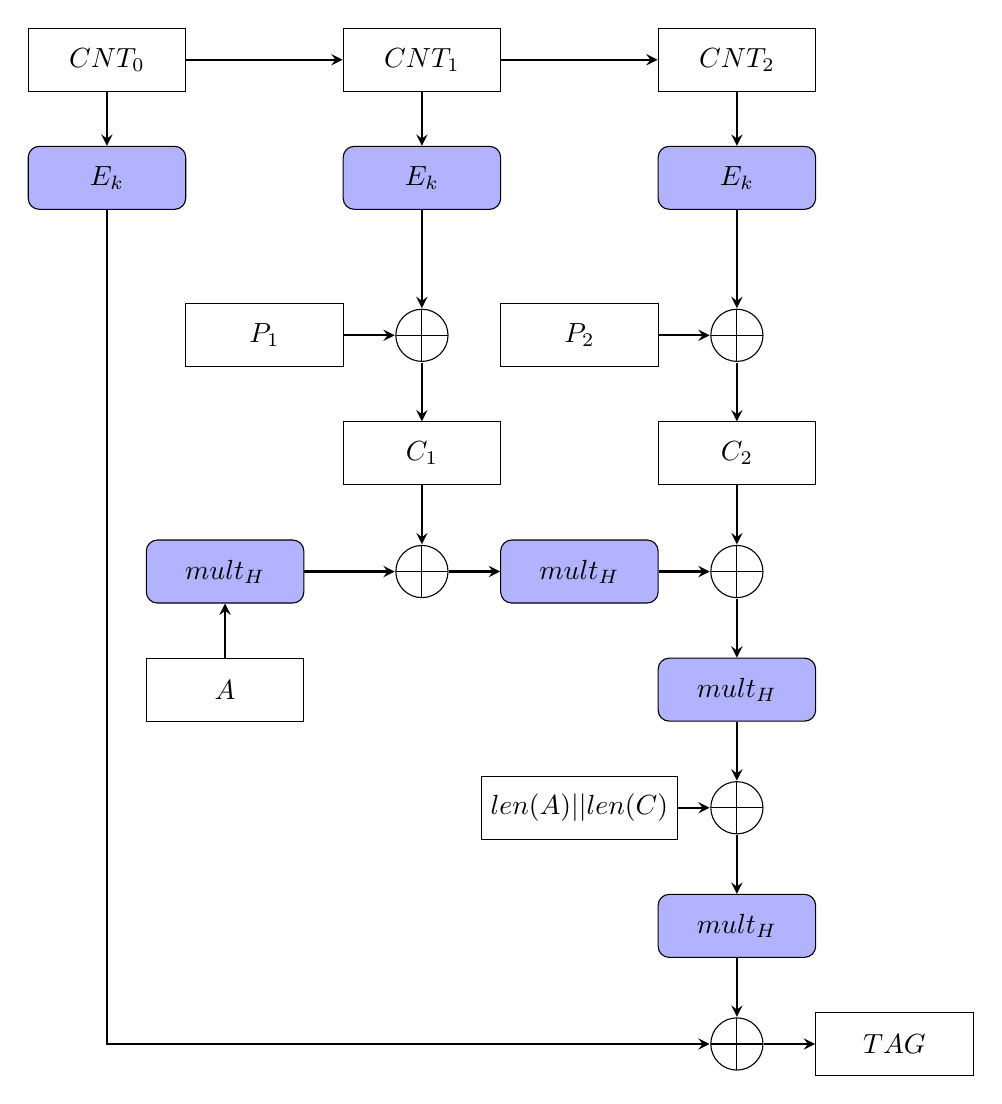
\begin{tikzpicture}
    \node (cnt0) [block]  {$CNT_0$};
    \node (cnt1) [block, right of=cnt0, xshift=3cm]  {$CNT_1$};
    \node (cnt2) [block, right of=cnt1, xshift=3cm]  {$CNT_2$};
    \node (enc0) [function, below of=cnt0, yshift=-0.5cm] {$E_k$};
    \node (enc1) [function, below of=cnt1, yshift=-0.5cm] {$E_k$};
    \node (enc2) [function, below of=cnt2, yshift=-0.5cm] {$E_k$};
    \node (xor11) [XOR, below of=enc1, scale=2, yshift=-0.5cm] {};
    \node (xor12) [XOR, below of=enc2, scale=2, yshift=-0.5cm] {};
    \node (pt1) [block, left of=xor11, xshift=-1cm] {$P_1$};
    \node (pt2) [block, left of=xor12, xshift=-1cm] {$P_2$};
    \node (ct1) [block, below of=xor11, yshift=-0.5cm] {$C_1$};
    \node (ct2) [block, below of=xor12, yshift=-0.5cm] {$C_2$};
    \node (xor21) [XOR, below of=ct1, scale=2, yshift=-0.25cm] {};
    \node (xor22) [XOR, below of=ct2, scale=2, yshift=-0.25cm] {};
    \node (mult1) [function, left of=xor21, xshift=-1.5cm] {$mult_H$};
    \node (mult2) [function, right of=xor21, xshift=1cm] {$mult_H$};
    \node (mult3) [function, below of=xor22, yshift=-0.5cm] {$mult_H$};
    \node (auth) [block, below of=mult1, yshift=-0.5cm] {$A$};
    \node (xor31) [XOR, below of=mult3, scale=2, yshift=-0.25cm] {};
    \node (len) [block, left of=xor31, xshift=-1cm] {$len(A) || len(C)$};
    \node (mult4) [function, below of=xor31, yshift=-0.5cm] {$mult_H$};
    \node (xor41) [XOR, below of=mult4, scale=2, yshift=-0.25cm] {};
    \node (tag) [block, right of=xor41, xshift=1cm] {$TAG$};

    \draw [arrow] (cnt0) -- (cnt1);
    \draw [arrow] (cnt1) -- (cnt2);
    \draw [arrow] (cnt0) -- (enc0);
    \draw [arrow] (cnt1) -- (enc1);
    \draw [arrow] (cnt2) -- (enc2);
    \draw [arrow] (enc0) |- (xor41);
    \draw [arrow] (enc1) -- (xor11);
    \draw [arrow] (enc2) -- (xor12);
    \draw [arrow] (pt1) -- (xor11);
    \draw [arrow] (pt2) -- (xor12);
    \draw [arrow] (xor11) -- (ct1);
    \draw [arrow] (xor12) -- (ct2);
    \draw [arrow] (ct1) -- (xor21);
    \draw [arrow] (ct2) -- (xor22);
    \draw [arrow] (mult1) -- (xor21);
    \draw [arrow] (auth) -- (mult1);
    \draw [arrow] (xor21) -- (mult2);
    \draw [arrow] (mult2) -- (xor22);
    \draw [arrow] (xor22) -- (mult3);
    \draw [arrow] (mult3) -- (xor31);
    \draw [arrow] (len) -- (xor31);
    \draw [arrow] (xor31) -- (mult4);
    \draw [arrow] (mult4) -- (xor41);
    \draw [arrow] (xor41) -- (tag);
  \end{tikzpicture}
  \caption{Schematic of AES-GCM. Whereas the $E_k$ blocks apply
AES-encryption with the key $k$. The $mult_H$ blocks apply a multiplication in
the Galois-field. $A$ represents a block of authenticated data, which is added
to the MAC $TAG$ but not encrypted.} \label{fig:aesgcm}
\end{figure}

Following steps describe how AES-GCM is used to encrypt data:

\begin{enumerate}
  \item The initialisation vector $IV$ of 96 bits is generated.
  \item The counters $CNT_i$ of 128 bits are generated by $CNT_i = IV \parallel
cnt$, where $cnt = (i + 1) \bmod{2^{32}}$, for $i \in\{0 .. n\}$ and $n$
represents the number of plaintext blocks.
  \item The ciphertexts $C_i$ are generated by encrypting the counter values
$CNT_i$ and XORing it to the plaintext $P_i$, as $C_i = P_i \oplus E_k(CNT_i)$.
\end{enumerate}

To get the authentication tag $TAG$, the $GHASH$ function,
$GHASH(H, A, C) = X_{m+n+1}$, is applied. Where, $H$ is the hash key, computed
by encrypting 128 zero bits with the AES block cypher, $C$ is the ciphertext,
and $A$ is non-encrypted but authenticated data. Figure~\ref{fig:aesgcm}
shows how the $GHASH$ is computed for one block of authenticated data and two
blocks of plaintext. Following steps describes the computation of the $TAG$:

\begin{enumerate}
  \item The Galois field multiplication is applied to the block of
authenticated data. $R_0 = mult_H(A_1)$.
  \item The result of this is XORed to the first ciphertext. The output
of this XOR is again multiplied in the Galois field. $R_1 = mult_H(R_0 \oplus
C_1)$.
  \item This output is then XORed to the second ciphertext and again
multiplied. $R_2 = mult_H(R_1 \oplus C_2)$
  \item Then the length of the authenticated data and the ciphertext is
added. $R_3 = mult_H(R_2 \oplus (len(A) \parallel len(C)))$
  \item The hash key is added in the end to form the tag $TAG$. $TAG = H \oplus
mult_H(R_3)$.
\end{enumerate}

The authenticated tag $TAG$ can therefore be found by solving the polynomial
$g(X) = A_{1}X^{m+n+1} + \cdots + A_{m}X^{n+2} + C_{1}X^{n+1} + \cdots +
C_{n}X^2 + LX + S$, as $g(H) = TAG$. Where $L$ is the combined length of $A$
and $C$, and $S$ is the nonce plus the counter. We refer to the NIST
standard about AES-GCM~\cite{gcmnist} for more details.

\paragraph{The OpenSSL source code} is structured in a way that each part of a
cypher is implemented on its own. For our thesis and analysation we want to
refer to version \texttt{1.1.0g} of OpenSSL\cite{opensslsource}. The AES-GCM
code part is located at \texttt{crypto/evp/e\_aes.c}. The structures used by the
cypher are defined in \texttt{crypto/evp/evp\_locl.h},
\texttt{crypto/include/internal/evp\_int.h} and \texttt{ssl/ssl\_locl.h}. The
file \texttt{crypto/evp/evp\_lib.c} shows the implementation for the creation of
the cypher data.

\subsubsection{AES-GCM Nonce Reuse Attack}

Joux\cite{NISTGCMcomment} calls his attack against GCM "a forbidden attack"
because in cryptography the uniqueness of nonces is seen as given.
Böck~\etal~\cite{gcmnonceattack} describe how relevant nonce reuse still is in
real-world application and why clear definitions for nonces in protocols are
needed.

We look at the simplified attack of Joux\textquotesingle s
comment~\cite{NISTGCMcomment}, described by Böck~\etal~\cite{gcmnonceattack}.
Assuming that the same nonce is used for two messages, consisting of just a
single ciphertext block and no authenticated data. Also,  we note that all
values besides $S$ are known to the attacker:

\[g_1(X) = C{_{1}X^2 \oplus L_1X \oplus S}\]
\[g_2(X) = C{_{2}X^2 \oplus L_2X \oplus S}\]

We add the tag $TAG$ to each polynomial to get $g_i'(X)$ as follows:

\[g_1'(X) = C{_{1}X^2 \oplus L_1X \oplus S \oplus T_1}\]
\[g_2'(X) = C{_{2}X^2 \oplus L_2X \oplus S \oplus T_2}\]

Knowing that $g_x'(H) = 0$, because $g_x(H) = T_x$, we combine those two
formulas to following polynomial:

\[g_{1+2}'(X) = (C_{1} + C_{2})X^2 + (L_1 + L_2)X + T_1 + T_2\]

This polynomial results in $0$ at the point $h$, $g_{1+2}'(H) = 0$.
Therefore, an attacker can calculate a list of possible solutions for $H$.
With an increasing number of nonce reuses the number of possible values for $H$
decreases.

\section{Software-based Microarchitectural Attacks}

Attacks against desktop computers and mobile devices have been widespread over
the last couple of years. As programmers and vendors became more aware of
classic issues in such systems, attackers moved to other layers to find bugs and
security holes. One of these other layers is side-channel information leakage.
Like Kelsey~\etal\cite{kelsey1998side} showed how little information was needed
to break cryptographic cypher implementations. They used time, processor flags,
and power consumption as their sources to break various implementations. But not
only cryptography was affected by side-channel attacks. As
Weinberg~\etal\cite{weinberg2011still} showed, it is also possible to gather
information about a users browser history by using side-channels.

\subsection{Caches}

Vendors of processors introduced the principle of caching to memory management
to speed up access times for memory. Hardware components closer to the computing
core holding a part of memory for future requests reply faster. In modern CPUs,
there are three or four levels of caching applied. As shown in
figure~\ref{fig:intelcache}, the design in Intel Kaby Lake assigns caches for
level one and two (L1, L2) to each core and the cores share the level three
cache (L3) between each other. L1 caches can be split up in a data and an
instruction cache. There might also be an L0 cache for micro-operations, as in
Intel Haswell.

Caches are updated on each memory access. Inclusive caching is a form of
managing the caches in a way where data stored on one level is also at lower
levels. The architecture defines if the CPU uses inclusive caches and which ones
are inclusive to others. The memory management part of the processor needs to
validate memory all the time to make sure memory accesses do not get wrong data
from other cache levels or the DRAM. Computation at rates of about four
gigahertz would not be possible without such caching mechanisms.

We refer to the Intel manual~\cite{intelsys} chapter 11.1 for more details about
cache management in modern CPUs.

\begin{figure}
  \centering
  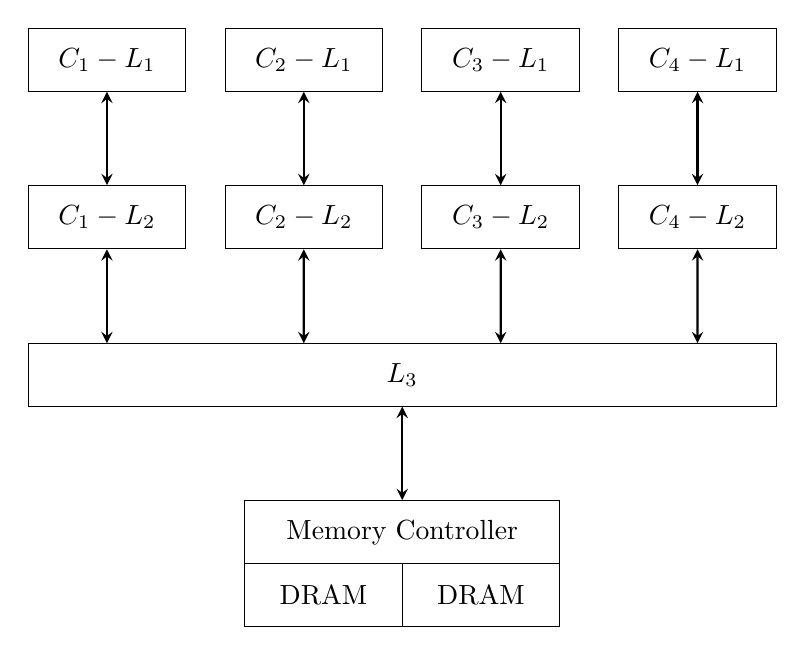
\begin{tikzpicture}
    % Level 1 caching blocks
    \node (C1L1) [block] {$C_1-L_1$};
    \node (C2L1) [block, right of=C1L1, xshift=1.5cm] {$C_2-L_1$};
    \node (C3L1) [block, right of=C2L1, xshift=1.5cm] {$C_3-L_1$};
    \node (C4L1) [block, right of=C3L1, xshift=1.5cm] {$C_4-L_1$};
    % Level 2 caching blocks
    \node (C1L2) [block, below of=C1L1, yshift=-1cm] {$C_1-L_2$};
    \node (C2L2) [block, right of=C1L2, xshift=1.5cm] {$C_2-L_2$};
    \node (C3L2) [block, right of=C2L2, xshift=1.5cm] {$C_3-L_2$};
    \node (C4L2) [block, right of=C3L2, xshift=1.5cm] {$C_4-L_2$};
    % Level 3 block
    \node (L3) [level3block, below of=C2L2, yshift=-1cm, xshift=1.25cm] {$L_3$};
    % Connections
    \draw [doublearrow] (C1L1) -- (C1L2);
    \draw [doublearrow] (C2L1) -- (C2L2);
    \draw [doublearrow] (C3L1) -- (C3L2);
    \draw [doublearrow] (C4L1) -- (C4L2);
    \draw [doublearrow] (C1L2) -- (0,-3.6cm);
    \draw [doublearrow] (C2L2) -- (2.5cm,-3.6cm);
    \draw [doublearrow] (C3L2) -- (5cm,-3.6cm);
    \draw [doublearrow] (C4L2) -- (7.5cm,-3.6cm);
    % Memory Controler and DDR3
    \node (MC) [mcblock, below of=L3, yshift=-1cm] {Memory Controller};
    \node (DDR31) [block, below of=MC, yshift=0.2cm, xshift=-1cm] {DRAM};
    \node (DDR32) [block, below of=MC, yshift=0.2cm, xshift=1cm] {DRAM};
    \draw [doublearrow] (L3) -- (MC);
  \end{tikzpicture}
  \caption{Schematic of Intel Kaby Lake caching architecture. Whereas $C_x$
represents each processing core and $L_x$ the level of the cache. Requests are
sent from the processing core to each memory storage, the one finding the
desired memory first will answer before the others. Caches get updated with
each request.} \label{fig:intelcache}
\end{figure}

\paragraph{Cache Attacks} are part of microarchitectural attacks, where
scientists have shown that caching also introduces security risks to systems.
Gruss~\etal\cite{gruss2015cache} showed how caches provide information by
measuring memory access-timings. They also showed how to automate attacks on
last-level caches. Knowledge gained from this kind of attack has also played
a role in the exploitation of the rowhammer bug.

\subsection{Rowhammer}

Technology is steadily changing and improving, with vendors of computer parts
being forced to produce cheaper and better hardware every year. For DRAM this
resulted in less quality management and a declining number of proper checks for
hardware faults. However, the industry produced smaller and faster memory chips.
These new chips need less space and energy to store electric load, which
represents data. Years after vendors introduced increased densities in DRAM to
the market, researchers like Kim~\etal\cite{rowhammergeneral} found a critical
bug in the chip design. With the little space and energy stored it was possible
to use changes of charges in memory rows to interfere with data of nearby cells.
This interference resulted in a change of bits in other memory rows.

This behaviour and bug then caused researchers to dig deeper into the
possibilities, and several attacks were found based on the rowhammer bug. For
example, Google\textquotesingle s "Project Zero"~\cite{projectzerorow} showed,
it is possible to use rowhammer for privilege escalation and sandbox escapes.
Van der Veen~\etal~\cite{drammer} state that this attack not only affects
desktop computers but also memory in mobile devices. In their work,
Gruss~\etal\cite{flipinthewall} show that flipping bits in memory has further
risks than previously thought and that Rowhammer defences need a general
overhaul. They state that the only solution is to fix the hardware.
Gruss~\etal~\cite{rowhammerjs} also showed that it is possible to trigger
bitflips from JavaScript.

\subsubsection{Design of Dynamic Random-Access Memory (DRAM)}

Random-access memory is designed to store information as bits. A simplified view
of RAM is a circuit containing amplifiers, one-bit storage cell matrix, an
address decoder and buffers for input and output of the memory.
Figure~\ref{fig:DRAMscheme} shows a simple schematic of a DRAM module. The
storage matrix is a two-dimensional array of one-bit storage cells. Accesses to
DRAM do not happen per bit but per row. The size of a row depends on the DRAM
design, but it is usually a multiple of the word size. In modern systems, rows
are larger than 64 kilobytes. The CPU sends requests for memory to the
controller which then translates it to a sequence, where first the column
entries to read are set via the bit lines and then the desired row via the word
lines. DRAM chips have many memory arrays and controllers which a data bus
connects with the processor.

A one-transistor (1-T) memory cell, as seen in figure~\ref{fig:1Tstorage}, is
used to store a single bit. To access memory, first, the desired bit lines are
charged with $\frac{V_{CC}}{2}$, then the word line is also charged to switch on
the transistors. An amplifier is then used to detect changes of charge on the
bit lines. A discharged capacitor would cause the voltage on the bit line to
drop, whereas a charged capacitor would raise the voltage to its load. If a
charged or discharged capacitor represents true or false for the bit state,
depends on the design of the DRAM chip. Writing the bits works in a similar way,
where the bit lines of a row are either set to $V_{CC}$ or $0$, and then the
word line is used to switch on the capacitors on the row, making the capacitors
change their charge to the level of the connected bit line.

The capacitor used for the 1-T cell will either lose load over time or on
reading access. Therefore, these capacitors need to be periodically refreshed.
The JEDEC standard~\cite{jedec} sets the refresh cycle to a 64-millisecond
interval. For a usual chip with $8192$ rows, this means a refresh happens all
$7,8$ microseconds. The easiest way to do this is by reading a bit and writing
the response back to it. In the DRAM design, it is possible to refresh each row
at a time with a RAS without the following CAS. With this refresh cycle, the
chip needs to hold the information which was the last refreshed row. Some DRAM
designs, therefore, implement a so-called row refresh pointer holding this
information.

\begin{figure}
  \centering
  \begin{circuitikz}
  \ctikzset{label/align = smart}
  \draw
  (0,0) to[short, l_=$bit\ line$] (0,-4)
  (-1,-1) to[short, l^=$word\ line$] (4,-1)
  (1,-2) node[nmos, rotate=-90] (mos) {}
  (mos.gate) node[anchor=north] {}
  (mos.drain) node[anchor=east] {}
  (mos.source) node[anchor=west] {}
  ;
  \draw
  (mos.gate) to[short] (1,-1)
  (mos.source) to[short] (0,-2)
  ;
  \draw
  (mos.drain) to[short] (2,-2)
  (2,-3) node[rground] (A) {}
  node[anchor=west, yshift=-0.4cm, xshift=0.2cm] {} to[pC, l_=$C$] (2,-2)
  ;
  \end{circuitikz}
  \caption{Schematic of a 1-T memory storage element. The capacitor $C$ is used
to store information. The transistor makes it possible to access the storage by
applying charge on the connected lines. Depending on the voltage used it is a
read or a write access.}
  \label{fig:1Tstorage}
\end{figure}

\begin{figure}
  \centering
  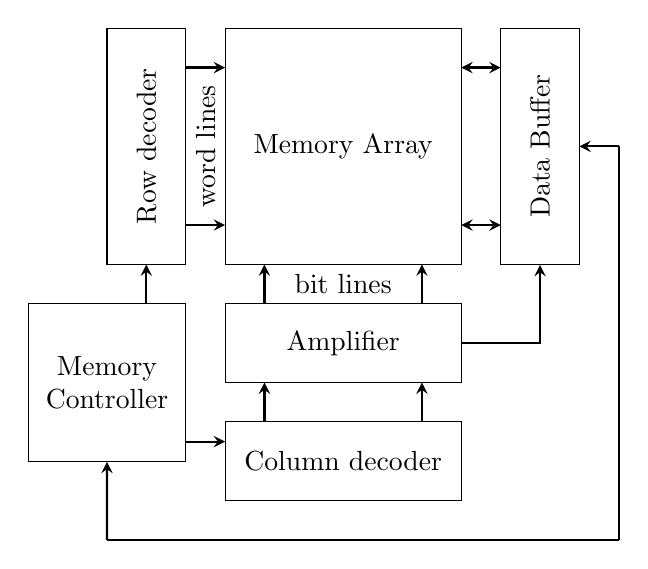
\begin{tikzpicture}
  %blocks
  \node (arr) [memarray]  {Memory Array};
  \node (rowdec) [memfunc, left of=arr, rotate=90, yshift=1.5cm] {Row decoder};
  \node (amp) [memfunc, below of=arr, yshift=-1.5cm] {Amplifier};
  \node (coldec) [memfunc, below of=amp, yshift=-0.5cm] {Column decoder};
  \node (memcon) [memcon, left of=amp, align=center, xshift=-2cm,
                  yshift=-0.5cm] {Memory \\ Controller};
  \node (buf) [memfunc, right of=arr, rotate=90, yshift=-1.5cm] {Data Buffer};
  %connections
  \draw [arrow] (amp) -| (buf);
  % memcon -> rowdec
  \draw [arrow] (-2.5,-2) -- (-2.5,-1.5);
  % memcon -> coldec
  \draw [arrow] (-2,-3.75) -- (-1.5,-3.75);
  % coldec -> amp
  \draw [arrow] (-1,-3.5) -- (-1,-3);
  \draw [arrow] (1,-3.5) -- (1,-3);
  % amp -> arr
  \draw [arrow] (-1,-2) -- (-1,-1.5);
  \draw [arrow] (1,-2) -- (1,-1.5);
  \node at (0,-1.75) {bit lines};
  % rowdec -> arr
  \draw [arrow] (-2,-1) -- (-1.5,-1);
  \draw [arrow] (-2,1) -- (-1.5,1);
  \node at (-1.75,0) [rotate=90] {word lines};
  % arr <-> buf
  \draw [doublearrow] (1.5,-1) -- (2,-1);
  \draw [doublearrow] (1.5,1) -- (2,1);
  % memcon <-> buf
  \draw [arrow] (-3,-5) -- (memcon.south);
  \draw [line] (-3,-5) -- (3.5,-5);
  \draw [line] (3.5,-5) -- (3.5,0);
  \draw [arrow] (3.5,0) -- (3,0);
  \end{tikzpicture}
  \caption{Schematic of a single DRAM module. The memory controller is managing
the data buffer to fill or read the buffer via a bus connection to the CPU. The
decoders are used to make sure the correct bits are accessed. The amplifier is
used because the bit voltage differences are usually too small to change the
memory in the buffer directly.}
  \label{fig:DRAMscheme}
\end{figure}

\subsubsection{Introducing bitflips to DRAM}

Kim~\etal\cite{rowhammergeneral} show how it is possible to cause bits to flip
inside memory by correct access patterns. They use two rows as so-called
aggressors, and one as target row. As the code in
listing~\ref{lst:rowhammercode} shows, the two aggressor rows are repeatedly
read, causing memory accesses in the DRAM. The changes in electrical charge
caused by the read accesses will by chance interfere with the loads in the
target row and change content there. The \texttt{clflush} instructions are used
to empty the memory in the used cache lines, causing the System to access the
DRAM for each read instead of getting the value out of the cache. These accesses
happen fast enough so that the refresh cycle of the DRAM cannot ensure that the
capacitors hold enough voltage.

\begin{minipage}{\linewidth}
\begin{lstlisting}[
  label={lst:rowhammercode},
  style=nasm,
  caption={Code to trigger the rowhammer bug, as of
Kim~\etal\cite{rowhammergeneral}. The preating accesses to the aggressor
locations cause bitflips in a third victim row. The \texttt{CFLUSH} is
neededed to make sure the DRAM rows are accessed directly. According to
Project Zero\cite{projectzerorow} the \texttt{mfence} is not needed and even
lowered the number of flips.},]
code1a:
  mov (X), %eax
  mov (Y), %ebx
  clflush (X)
  clflush (Y)
  mfence
  jmp code1a
\end{lstlisting}
\end{minipage}

The memory addresses to be accessed to gain the rows next to each other are hard
to find. Linux provides a file, \texttt{/proc/<PID>/pagemap}, where physical
positioning is stored. Some systems allow huge pages, where two megabytes of
memory are used contiguously. These two megabytes will use more than one row,
other than normal pages with the size of four kilobytes. In the paper,
Kim~\etal~\cite{rowhammergeneral} use addresses calculated based on their
knowledge of physical address mapping used by common CPU vendors.

Project Zero~\cite{projectzerorow} show how it is possible to use rowhammer to
gain privilege escalation on a standard \texttt{x86\_64} CPU and an escape from
a sandbox. After vendors of operating systems started to introduce
countermeasures, scientists like Gruss~\etal\cite{rowhammerjs}, came up with
further, improved attacks making use of the rowhammer bug. They show that it is
not only possible to use rowhammer to gain privilege escalation by flips in
page-tables but also by targeting bits in the file-cache of the operating
system.
%}}}

%% vim:foldmethod=expr
%% vim:fde=getline(v\:lnum)=~'^%%%%\ .\\+'?'>1'\:'='
%%% Local Variables:
%%% mode: latex
%%% mode: auto-fill
%%% mode: flyspell
%%% eval: (ispell-change-dictionary "en_US")
%%% TeX-master: "main"
%%% End:
